% In this section, the layer is described in terms of the hardware and software design. Specific implementation details, such as hardware components, programming languages, software dependencies, operating systems, etc. should be discussed. Any unnecessary items can be omitted (for example, a pure software module without any specific hardware should not include a hardware subsection). The organization, titles, and content of the sections below can be modified as necessary for the project.
The Degree Planner Firebase Layer consists of two subsystems, Authentication and Firestore Database. It is reposible for authenticating the user and retrieving their information. The database function will return null unless the user has been authenticated with Firebase.

\subsection{Layer Hardware}
% A description of any involved hardware components for the layer. For example, if each subsystem is a software process running on an embedded computer, discuss the specifics of that device here. Do not list a hardware component that only exists at the subsystem level (include it in the following sections).
The Firebase layer is dependent on Firebase servers hosted by Google.

\subsection{Layer Operating System}
% A description of any operating systems required by the layer.
Google's Firebase does not publish what operating system their servers run on.

\subsection{Layer Software Dependencies}
% A description of any software dependencies (libraries, frameworks, etc) required by the layer.
The Firebase layer uses JavaScript/TypeScript to make requests to Firebase. It is dependent on the firebase-core package. This package is required for both subsystem's software dependencies.

\subsection{Authentication Subsystem}
Describe at a high level the purpose and basic design of this subsystem. Is it a piece of hardware, a class, a web service, or something else? Note that each of the subsystem items below are meant to be specific to that subsystem and not a repeat of anything discussed above for the overall layer.

%%%%%%%%%%%%%%%%%%%%%%%%%%%%%%%%%%%%%%%%%%%%%%%%%%%%%%%%%%
%  BE SURE TO UPDATE THE IMAGE CAPTION
\begin{figure}[h!]
	\centering
	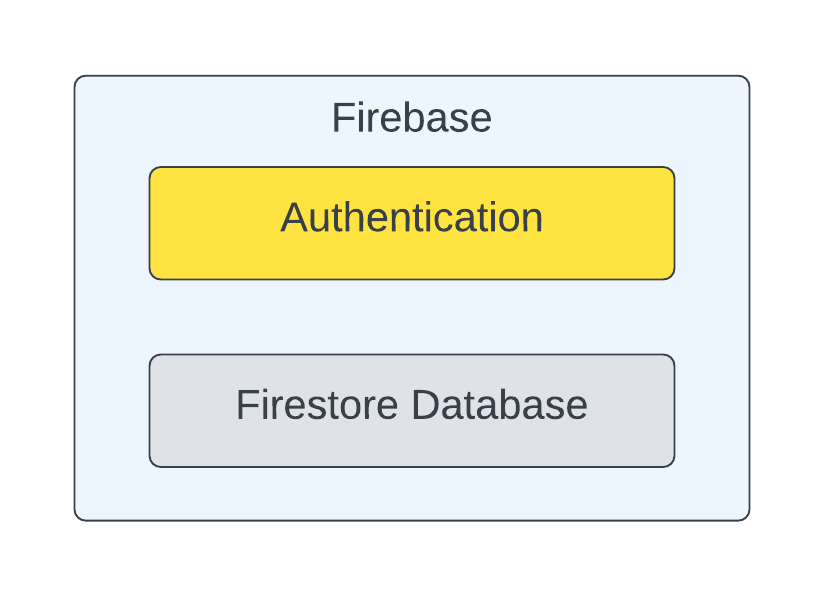
\includegraphics[width=0.60\textwidth]{images/DDS_Diagram_Firebase_Authentication} % Image
	\caption{Diagram of the Firebase layer with the Authentication subsystem selected}
\end{figure}

% \subsubsection{Subsystem Hardware}
% A description of any involved hardware components for the subsystem.

% \subsubsection{Subsystem Operating System}
% A description of any operating systems required by the subsystem.

\subsubsection{Subsystem Software Dependencies}
% A description of any software dependencies (libraries, frameworks, design software for mechanical parts or circuits, etc) required by the subsystem.
The Authentication Subsystem is dependent on the firebase-auth package to authenticate the user before they can use the website.

\subsubsection{Subsystem Programming Languages}
% A description of any programming languages used by the subsystem.
The Authentication Subsystem is programmed using TypeScript.

\subsubsection{Subsystem Data Structures}
% A description of any classes or other data structures that are worth discussing for the subsystem. For example, data being transmitted from a microcontroller to a PC via USB should be first be assembled into packets. What is the structure of the packets?
The Authentication Subsystem has all authentication functions in one file, and each function is exported. This allows for the server to take advantage of tree shaking, which means only code needed is imported and not the entire file.

% \subsubsection{Subsystem Data Processing}
% A description of any algorithms or processing strategies that are worth discussing for the subsystem. If you are implementing a well-known algorithm, list it. If it is something unique to this project, discuss it in greater detail.

\subsection{Firestore Database Subsystem}
% Describe at a high level the purpose and basic design of this subsystem. Is it a piece of hardware, a class, a web service, or something else? Note that each of the subsystem items below are meant to be specific to that subsystem and not a repeat of anything discussed above for the overall layer.
The Firestore Database Subsystem is responsible for retrieving user information, their chosen courses, and a list of all courses from the Firebase Firestore Database.

%%%%%%%%%%%%%%%%%%%%%%%%%%%%%%%%%%%%%%%%%%%%%%%%%%%%%%%%%%
%  BE SURE TO UPDATE THE IMAGE CAPTION
\begin{figure}[h!]
	\centering
	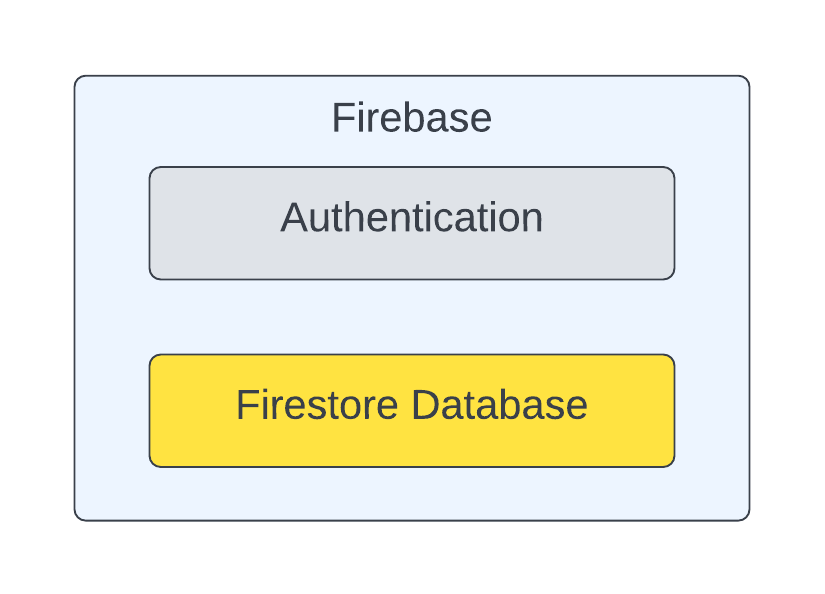
\includegraphics[width=0.60\textwidth]{images/DDS_Diagram_Firebase_Firestore_Database} % Image
	\caption{Diagram of the Firebase layer with the Firestore Database subsystem selected} % Caption
\end{figure}

% \subsubsection{Subsystem Hardware}
% A description of any involved hardware components for the subsystem.

% \subsubsection{Subsystem Operating System}
% A description of any operating systems required by the subsystem.

\subsubsection{Subsystem Software Dependencies}
% A description of any software dependencies (libraries, frameworks, design software for mechanical parts or circuits, etc) required by the subsystem.
The Firestore Database Subsystem is dependent on the firebase-firestore package to make database queries to the Firestore Database.

% \subsubsection{Subsystem Programming Languages}
% A description of any programming languages used by the subsystem.

\subsubsection{Subsystem Data Structures}
% A description of any classes or other data structures that are worth discussing for the subsystem. For example, data being transmitted from a microcontroller to a PC via USB should be first be assembled into packets. What is the structure of the packets?
The Firebase Database Subsystem has all authentication functions in one file, and each function is exported. This allows for the server to take advantage of tree shaking, which means only code needed is imported and not the entire file.

\subsubsection{Subsystem Data Processing}
% A description of any algorithms or processing strategies that are worth discussing for the subsystem. If you are implementing a well-known algorithm, list it. If it is something unique to this project, discuss it in greater detail.
The Firebase Database Subsystem processes the data received from Firestore and converts it to Class Objects to take advantage of static analysis.

The subsystem converts the JSON string received from the all courses list in Firestore and converts it to a list of Courses objects.

The subsystem converts the user information stored in Firestore and converts it to the object UserData. When processing the user information, it also converts the user's chosen classes to the ChosenCourse object. The ChosenCourse object is a minified version of Course with an id reference to the Course object with the full details.
